\documentclass[13pt,letterpaper,fleqn]{article}

%       amslatex provides nice math extensions for typesetting mathematics
\usepackage{amsmath}
\usepackage{amsfonts}
\usepackage{tmmaths}
\usepackage{sympytex}

%       pstricks provides powerful environments for incorporating postscript into a
%       TeX/LaTeX document. You must have a postscript printer and a package like
%       dvips to convert the DVI file to a PS file.
%\usepackage{pst-all}
%\usepackage{pstricks,pst-plot}
%\usepackage{pst-coil,pst-node}

%  This package provides native tex support for numbered grids. The syntax is:
%  \graphpaper[spc](x_lowleft,y_lowleft)(x_upperright,y_upperright)

%\usepackage{graphpap}
%\usepackage{float}

%  The package below must be initialized with "\initfloatingfigs" immediately after the
%  "\begin{document} command.
%\usepackage{floatfig}

\usepackage{graphicx}
\graphicspath{{i:/mytex/graphics}}
\DeclareGraphicsExtensions{.ps,.eps}

%       tst is a package for the creation of exams, quizzes and tests. the include
%       file mathstuf (see below) provides many abbreviations for these environments.
%\usepackage{tst}

%       epsfig is a package which provides for the inclusion of Encapsulated PostScript
%       files in a document.
%\usepackage{epsfig}
%\usepackage{epic,eepic}
\include{mathstuf}
\usepackage[total={7.25in,10in},top=0.25in,left=0.75in,includehead]{geometry}
\usepackage{fancyhdr}
\pagestyle{fancy}
\lhead{Math 253}
\rhead{\large Name\makebox[2in]{\hrulefill}}
\chead{\LARGE Exploration 19}
%\lfoot{\today}
\cfoot{}
%\rfoot{\thepage}
\renewcommand{\headrulewidth}{0.4pt}
\renewcommand{\footrulewidth}{0.4pt}
\setlength{\parindent}{0pt}
\setlength{\parskip}{2ex}

\newcounter{tf}[enumi]
\newenvironment{tf}[0]{\begin{list}%
{\alph{tf}. \makebox[5em]{True\hfill False}}%
{\usecounter{tf}\setlength{\labelwidth}{7em}%
\setlength{\leftmargin}{3.5cm}%
\setlength{\labelsep}{1cm}}}%
{\end{list}}

%\usepackage{epic,eepic}
\newcommand{\numline}{%
%\newcounter{mark}%
%\setcounter{mark}{-1}%
\setlength{\unitlength}{0.1in}%
\begin{picture}(0,0)%
\thicklines%
\put(0,0){\line(1,0){60}}%
\multiput(0,0)(10,0){7}{\line(0,-1){1}%
\makebox(0,-1.5)[t]{\arabic{mark}}\stepcounter{mark}}%
%
\thinlines%
\multiput(0,0)(5,0){12}{\line(0,-1){0.5}}%
\multiput(0,0)(1,0){60}{\line(0,-1){0.3}}%
%\put(-5,265){\makebox(0,0)[l]{{\bf cm}}}%
\end{picture}}%

\newcommand{\ds}{\displaystyle}
\usepackage{amsfonts}


\let\oldhat\hat
\renewcommand{\hat}[1]{\oldhat{\boldsymbol{\mathbf{#1}}}}
\newcommand{\lv}[1]{\ensuremath{\left\langle #1 \right\rangle}}
\renewcommand{\i}{\ensuremath{\hat{\imath}}}
\renewcommand{\j}{\ensuremath{\hat{\jmath}}}
\renewcommand{\k}{\ensuremath{\mathbf{\oldhat{k}}}}
\newcommand{\ora}[1]{\ensuremath{\overrightarrow{#1}}}
\renewcommand{\vec}[1]{\ensuremath{\pmb{#1}}}
\renewcommand{\v}[1]{\ensuremath{\vec{#1}}}
\newcommand{\abs}[1]{\ensuremath{\lvert #1 \rvert}}
\renewcommand{\deg}{\ensuremath{{}^\circ}}

\usepackage{tabularx}
\usepackage{paralist}
\newcommand{\red}[1]{\textcolor{red}{#1}}
\newcommand{\blue}[1]{\textcolor{blue}{#1}}
% \newcommand{\ans}[1]{\quad\fbox{answer: \red{#1}}}
\newcommand{\ans}[1]{\mbox{{\bf Ans:} \blue{#1}}}
\newcommand{\dd}[2][]{\ensuremath{\frac{\text{d}#1}{\text{d}#2}}}
\newcommand{\eval}[2]{\ensuremath{\left.#1\right|_{#2}}}
\newcommand{\proj}[2]{\ensuremath{\text{proj}_{\v{#2}}\v{#1}}}

\usepackage{enumitem}
\usepackage{caption}
\usepackage{subcaption}

\renewcommand{\thefigure}{}

\begin{document}
\section*{Partial Derivatives}
Let $w = f(x_1,\ldots,x_n)$ be a function of the $n$ independent variables $x_1,\ldots,x_n$. The $n$ (first) partial derivatives ($f_{x_i}$ for $i=1,\ldots,n$)\footnote{Other notations for these (first) derivatives are $w_{x_i}$, $\partial f/\partial x_i$, $\partial w/\partial x_i$ and $D_{x_i}f$} of $f$ are obtained by differentiating $f$ with respect to one of its inputs, while treating all the other inputs as constants; The $n$ partial derivatives are the derivatives of $n$ single variable functions.

For example, the three (first) partial derivatives of the function $f(x,y,z) = 3x^2 y - 2xy^3 z^2 + y^2 z^5$ are: $f_x = 6xy - 2y^3 z^2$, $f_y = 3x^2 - 6xy^2 z^2 + 2y z^5$, and $f_z = -4xy^3 z + 5y^2 z^4$.
% description of a device with many knobs

We can gain a geometric understanding of the (first) partial derivatives of a function $f(x,y)$ of two input variables as the slopes of tangent lines to the traces of the graph of $f$ in the planes $x = a$ and $y = b$, where $a$ and $b$ are constants.

Consider the graph of $z = f(x,y) = 4 - \frac{1}{4}\left(x^2 - \frac{1}{5}y^3\right)$ and its traces in the planes $y = -3$ and $x = 1$ below.
\begin{figure*}[ht!]
 \centering
 \begin{subfigure}[t]{0.33\textwidth}
  \centering
  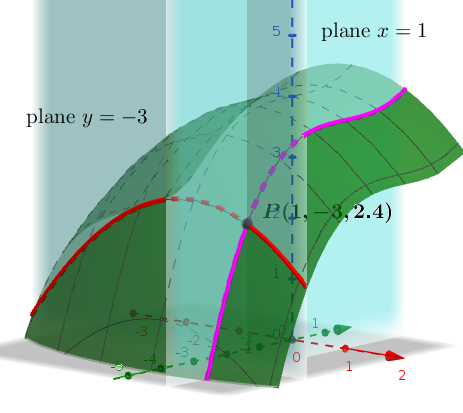
\includegraphics[width=0.8\linewidth]{img/Surface.png}
  \caption{Graph of $f(x,y)$}
  \label{f}
 \end{subfigure}
 \begin{subfigure}[t]{0.33\textwidth}
  \centering
  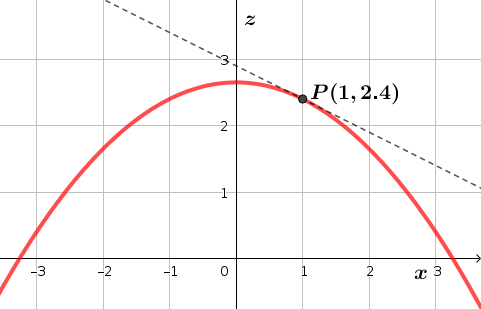
\includegraphics[width=0.8\linewidth]{img/parabola_trace.png}
  \caption{Trace of $f$ in the plane $y=-3$}
  \label{fx}
 \end{subfigure}
 \begin{subfigure}[t]{0.33\textwidth}
  \centering
  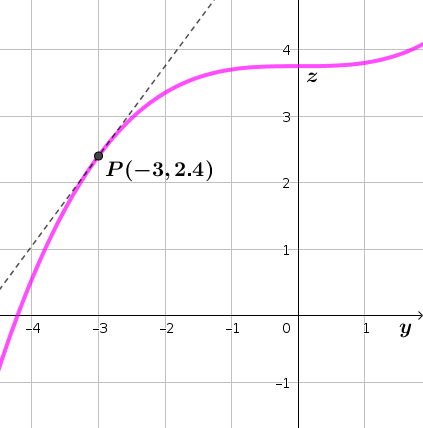
\includegraphics[width=0.8\linewidth]{img/cubic_trace.png}
  \caption{Trace of $f$ in the plane $x=1$}
  \label{fy}
 \end{subfigure}
 \caption*{}
\end{figure*}%
\subsection*{Problems}
\begin{enumerate}
 \item What is the equation of the trace depicted in figure (\ref{fx})?
 \item What is the equation of the trace depicted in figure (\ref{fy})?
 \item Use figures (\ref{fx}) and (\ref{fy}) to estimate the values of $z_x(1,-3)$ and $z_y(1,-3)$.
 \item Use the derivative of the function from problem 1 to find the exact value of $z_x(1,-3)$. How does the exact value compare to the approximation you found in problem 3?
 \item Use the derivative of the function from problem 2 to find the exact value of $z_y(1,-3)$. How does the exact value compare to the approximation you found in problem 3?
\end{enumerate}
\section*{A Physical Example}
Imagine a quantity of gas confined to a cylinder with a piston that can be used to compress or expand the gas\footnote{Similar to the cylinders and pistons in the engines of a gasoline powered car.}. If the gas is an ideal gas, the relationship between its pressure $P$ (in ``kilo Pascals'' kPa), volume $V$ (in liters L) and temperature $T$ (in Kelvin K) obey the ideal gas law
\begin{equation*}
 PV = nRT
\end{equation*}
where $n$ is the number of moles\footnote{A measure of the number of molecules in the cylinder} of gas, and $R$ is the ideal gas constant. This equation relates the three parameters $P$, $V$ and $T$. We can solve the equation for any one of the parameters in terms of the other two, giving us three different (but related) functions of two variables: $P(T,V)$, $V(T,P)$ and $T(V,P)$.
\subsection*{Problems}
Supposing that $nR = 10 \text{ L kPa/K}$
\begin{enumerate}
 \item Calculate $P_T(300, 2)$ and interpret its meaning.
 \item Calculate $P_V(300, 2)$ and interpret its meaning.
 \item Calculate $V_T(300, 5)$ and interpret its meaning.
 \item Calculate $V_P(300, 5)$ and interpret its meaning.
\end{enumerate}
\end{document}
